%!TEX TS-program = xelatex

% -- Document Class -----------------------------------------------------------

\documentclass[a4paper, 11pt]{article}

% -- Packages -----------------------------------------------------------------

% Language
\usepackage{polyglossia}
    \setmainlanguage{english}
    \setotherlanguage{german}
% Context sensitive quotation
\usepackage{csquotes}
% Citations
\usepackage[style=alphabetic, backend=biber]{biblatex}
    \addbibresource{References.bib}
% Caption support
\usepackage{caption}
% Customize enumerations
\usepackage{enumitem}
% Extend options for positioning floats
\usepackage{float}
% Support highlighting of certain parts of the text
\usepackage{framed}
% Support spaces in filenames
\usepackage{grffile}
% Tools for mathematical typesetting
\usepackage{mathtools}
% Headers & Footers
\usepackage[automark, nouppercase]{scrpage2}
% Emphasize text
\usepackage{soul}
% To change the format of titles
\usepackage{titlesec}
% Support for unicode math fonts
\usepackage{unicode-math}
% Extended color support
\usepackage[x11names]{xcolor}
% Extras for XƎTEX
\usepackage{xltxtra}
% Hyperlinks and pdf properties
\usepackage{hyperref}

% -- Color Definitions --------------------------------------------------------

% Background color for syntax highlighting
\definecolor{bgcolor}{rgb}      {1,     1,      1}

% Custom color definitions
\definecolor{aqua}{rgb}         {0,     0.56,   1}
\definecolor{bluegray}{rgb}     {0.22,  0.46,   0.84}
\definecolor{grape}{rgb}        {0.56,  0,      1}
\definecolor{lightgray}{rgb}	{0.94,	0.94,	0.94}
\definecolor{orchid}{rgb}       {0.41,  0.13,   0.55}
\definecolor{orange}{rgb}       {1,     0.54,   0}
\definecolor{silver}{rgb}       {0.57,  0.57,   0.57}
\definecolor{turquoise}{rgb}    {0,     0.86,   0.84}

% -- Macros -------------------------------------------------------------------

\newcommand{\Title}{Exercises}
\newcommand{\TitleDescription}{Computer Aided Verification}
\newcommand{\Version}{1}
\newcommand{\Subject}
    {Solutions for the exercises of the course Computer Aided Verification}
\newcommand{\KeyWords}{BDD, Kripke structure}
\newcommand{\LeftFooter}{\Title~—~\TitleDescription}

\newcommand{\AuthorOne}{René Schwaiger}
\newcommand{\MailOne}{\href{mailto:sanssecours@f-m.fm}{sanssecours@f-m.fm}}

% Syntax highlighting definitions
% Text
\newcommand{\hlstd}[1]{\textcolor{black}{#1}}
% Numbers
\newcommand{\hlnum}[1]{\textcolor{DarkOrchid4}{#1}}
\newcommand{\hlesc}[1]{\textcolor[rgb]{1,0,1}{#1}}
% Strings
\newcommand{\hlstr}[1]{\textcolor{SeaGreen3}{#1}}
\newcommand{\hlpps}[1]{\textcolor[rgb]{0.51,0.51,0}{#1}}
% Comments
\newcommand{\hlslc}[1]{\textcolor{aqua}{#1}}
\newcommand{\hlcom}[1]{\textcolor{aqua}{#1}}
\newcommand{\hlppc}[1]{\textcolor[rgb]{0,0.51,0}{#1}}
\newcommand{\hlopt}[1]{\textcolor[rgb]{0,0,0}{#1}}
\newcommand{\hllin}[1]{\textcolor[rgb]{0.33,0.33,0.33}{#1}}
% Keywords
\newcommand{\hlkwa}[1]{\textcolor{DodgerBlue3}{#1}}
\newcommand{\hlkwb}[1]{\textcolor[rgb]{0,0.34,0.68}{#1}}
\newcommand{\hlkwc}[1]{\textcolor{DarkOrchid4}{#1}}
% Functions
\newcommand{\hlkwd}[1]{\textcolor{orange}{#1}}

\newcommand{\codeinput}[1]
{
    \vskip 0.3 cm
    {\color{lightgray}\hrule}\vskip 0.3 cm
    {\fontsize{9pt}{11pt}\input{Code/#1}}
    \vskip 0.3 cm{\color{lightgray}\hrule}
    \vskip 0.3 cm
}

\newcommand{\code}[1]
{
    \hl{\texttt{#1}}
}

% -- Document Properties ------------------------------------------------------

% Background color for highlighted text
\sethlcolor{lightgray}

% No indentation after paragraphs
\setlength\parindent{0cm}

% Hyperref properties
\hypersetup
{
    pdftitle    = {\Title},
    pdfsubject  = {\Subject},
    pdfauthor   = {\AuthorOne},
    pdfkeywords = {\KeyWords},
    colorlinks  = true,
    linkcolor   = black,
    anchorcolor = black,
    citecolor   = silver,
    urlcolor    = orange
}

% -- Fonts --------------------------------------------------------------------

% Use same size for numbers and other text
\defaultfontfeatures{Numbers=Lining}

% Set fonts for document
\setmainfont[Mapping=tex-text]{Avenir Next}
\setsansfont[Mapping=tex-text]{Ubuntu}
\setmonofont[Scale=MatchLowercase]{Menlo}
\setmathfont{Asana-Math.otf}
\setmathfont[range=\mathtt, Scale=MatchLowercase]{Menlo}

% Define font styles
\newfontfamily\Zapfino{Zapfino}

% -- Header And Footers -------------------------------------------------------

% Use normal font instead of italic font for head
\renewcommand{\headfont}{\normalfont}

% Set headers and footers
\ihead{\headmark}
\ohead{}
\ifoot{\LeftFooter}
\ofoot{\thepage}

% Set height of head
\setlength{\headheight}{1.8\baselineskip}

% Set thickness of separation line in header, footer
\setheadsepline{0.5pt}
\setfootsepline{0.5pt}

% -- Titlepage ----------------------------------------------------------------

\pagestyle{empty}
\begin{document}

\begin{titlepage}
    \begin{center}
        % Title and title-description
        {\Huge\Zapfino\Title}
        \vskip 0.5cm
        {\color{aqua}\hrule}
        \vskip 0.5cm
        {\Large\textit\TitleDescription}
        \vskip 14cm
    \end{center}

    % Date and version number
    \begin{leftbar}
        \begin{tabular}{ll}
            \textbf{Author}  & \AuthorOne\\
            \textbf{Mail}    & \MailOne\\
            \textbf{Version} & \Version\\
            \textbf{Date}    & \today
        \end{tabular}
    \end{leftbar}

\end{titlepage}


% -- Table of Contents --------------------------------------------------------

% Set section format for table of contents
\titleformat{\section}{\sffamily\bfseries}{}{0pt}{}[{\color{aqua}\hrule}]

% Set separation of dots between name of section and page number to such a high
% value that there will be no points in the table of contents
\makeatletter \renewcommand{\@dotsep}{10000} \makeatother
% Use blank header and footer
\pagestyle{empty}
% Start on new page
\newpage
% The table of contents starts at the second page
\setcounter{page}{2}
% Set table of contents
\tableofcontents

% -- Section & Paragraph Style ------------------------------------------------

% Set format for section
\titleformat{\section}
    {\large\sffamily\bfseries}  % Large, bold, sans serif font for section
    {}                          % No format applied to whole title
    {0pt}                       % No separation between label and title
    {\thesection~·~}            % Start with section number
    [{\color{aqua}\hrule}]      % Underline with blue ruler

% Set format for other sections and paragraphs
% Color = orchid, Font = bold, sans serif
\titleformat*{\subsection}{\color{orchid}\sffamily\bfseries}
\titleformat*{\subsubsection}{\color{orchid}\sffamily\bfseries}
\titleformat*{\paragraph}{\color{orchid}\sffamily\bfseries}
\titleformat*{\subparagraph}{\color{orchid}\sffamily\bfseries}

% -- Page Style ---------------------------------------------------------------

% Start with text on a new page
\newpage
% Display headers and footers
\pagestyle{scrheadings}

% -- Text ---------------------------------------------------------------------

\section{Binary Decision Diagrams}

\subsection{Exercise 1}

Give a linear time algorithm for BDD isomorphism as defined on page 9.

\subsubsection{Solution}

The following code assumes the existence of the functions:

\begin{description}[style=multiline, leftmargin=3cm]
    \item[\texttt{is\_terminal(v)}] Returns \texttt{True} if \texttt{v} is a terminal vertex and \texttt{False} otherwise
\end{description}

\paragraph{Nonterminal Vertices}

\begin{description}[style=multiline, leftmargin=3cm]
    \item [\texttt{var(v)}] Returns the variable of a BDD vertex.
    \item [\texttt{low(v)}] Returns the “low” successor of the BDD vertex (v is set to 0)
    \item [\texttt{high(v)}] Returns the “high” successor of the BDD vertex (v is set to 1)
\end{description}

\paragraph{Terminal Vertices}

\begin{description}[style=multiline, leftmargin=3cm]
    \item[\texttt{high(v)}] Returns the value of v (Either 0 or 1)
\end{description}

\codeinput{isomorphic}

\newpage
\subsection{Exercise 2}

Show that the three operations on page 12 commute.

\subsubsection{Solution}

We have the following operations:

\begin{description}[style=multiline, leftmargin=3.6cm]
    \item[Remove duplicate terminals] Eliminate all but one terminal vertex with a given label and redirect all arcs to the eliminated vertices to the remaining one.
    \item[Remove duplicate nonterminals] If nonterminals $u$ and $v$ have $high(u)=high(v)$, $low(u)=low(v)$ and $high(u)=high(v)$, then eliminate one of the two vertices and redirect all incoming arcs to the other vertex.
    \item[Remove redundant test] If nonterminal vertex $v$ has $low(v)=high(v)$, then eliminate $v$ and redirect all incoming arcs to $low(v)$.
\end{description}

We now use the following abbreviations for these operations:

\begin{description}[style=multiline]
    \item[dt()] Remove duplicate terminals
    \item[dn()] Remove duplicate nonterminals
    \item[rt()] Remove redundant test
\end{description}

To show that these operations are commutative — the order of application does not matter – we need to show the following:

\begin{enumerate}
    \item $dt(dn(bdd)) = dn(dt(bdd))$
    \item $dt(rt(bdd)) = rt(dt(bdd))$
    \item $dn(rt(bdd)) = rt(dn(bdd))$
\end{enumerate}

$bdd$ describes an arbitrary binary decision diagram.

\paragraph{dt(dn(bdd)) = dn(dt(bdd))}

The only place where the order of operations could matter is on the bottom of the graph, where nonterminal nodes connect to terminal nodes. In the other case the operations work on different parts of the tree.\\

If we first remove duplicate nonterminal nodes, then theoretically we could remove one of the two terminal nodes, that we used if we first removed the duplicate terminals. Figure~\ref{fig:Figures_BDD_Removed_Terminals_And_Nonterminals} shows an example of this behaviour. This does however not change the semantics, since every terminal vertex $v$ with $value(v)=0$ is isomorphic to a vertex $u$ with $value(u)=0$. The same of course is true for terminal vertices that have a value of 1.

\begin{figure}[h]
  \centering
    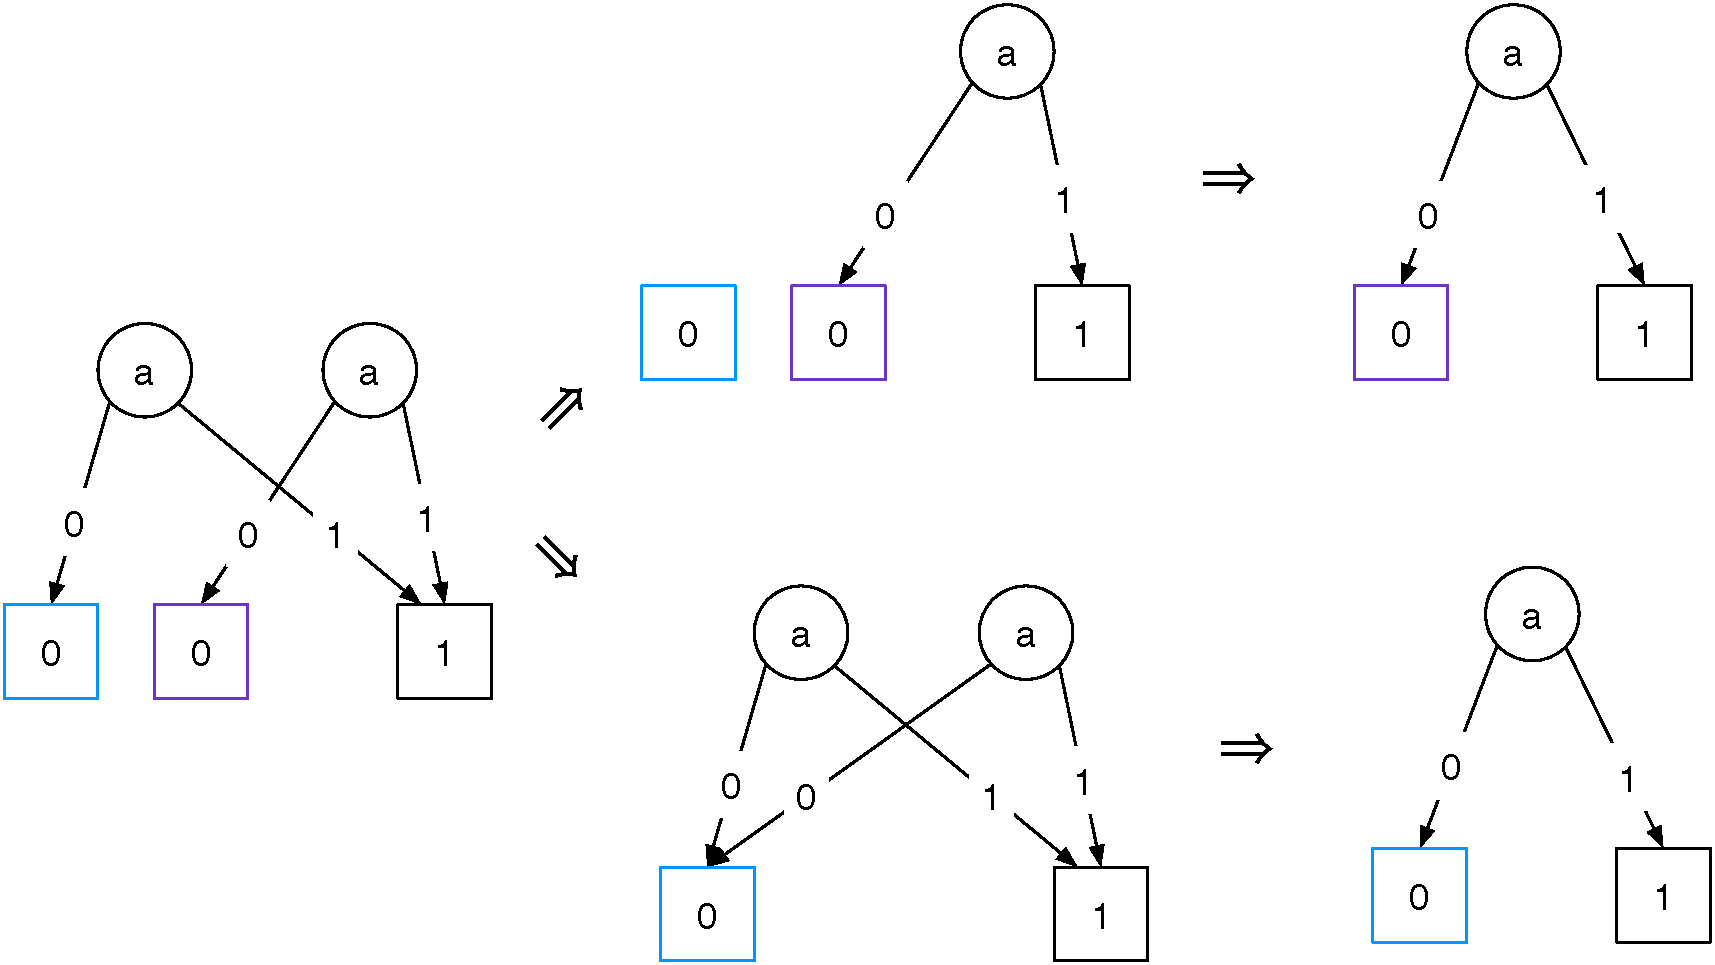
\includegraphics[width=.9\textwidth]{Figures/BDD Removed Terminals And Nonterminals.pdf}
  \caption{Removal of terminal and nonterminal nodes in a BDD}
  \label{fig:Figures_BDD_Removed_Terminals_And_Nonterminals}
\end{figure}

\paragraph{dt(rt(bdd)) = rt(dt(bdd))}

This case is similar to the one before. The only place where the order of the operations matter is at the bottom of the tree.

\begin{figure}[h]
  \centering
    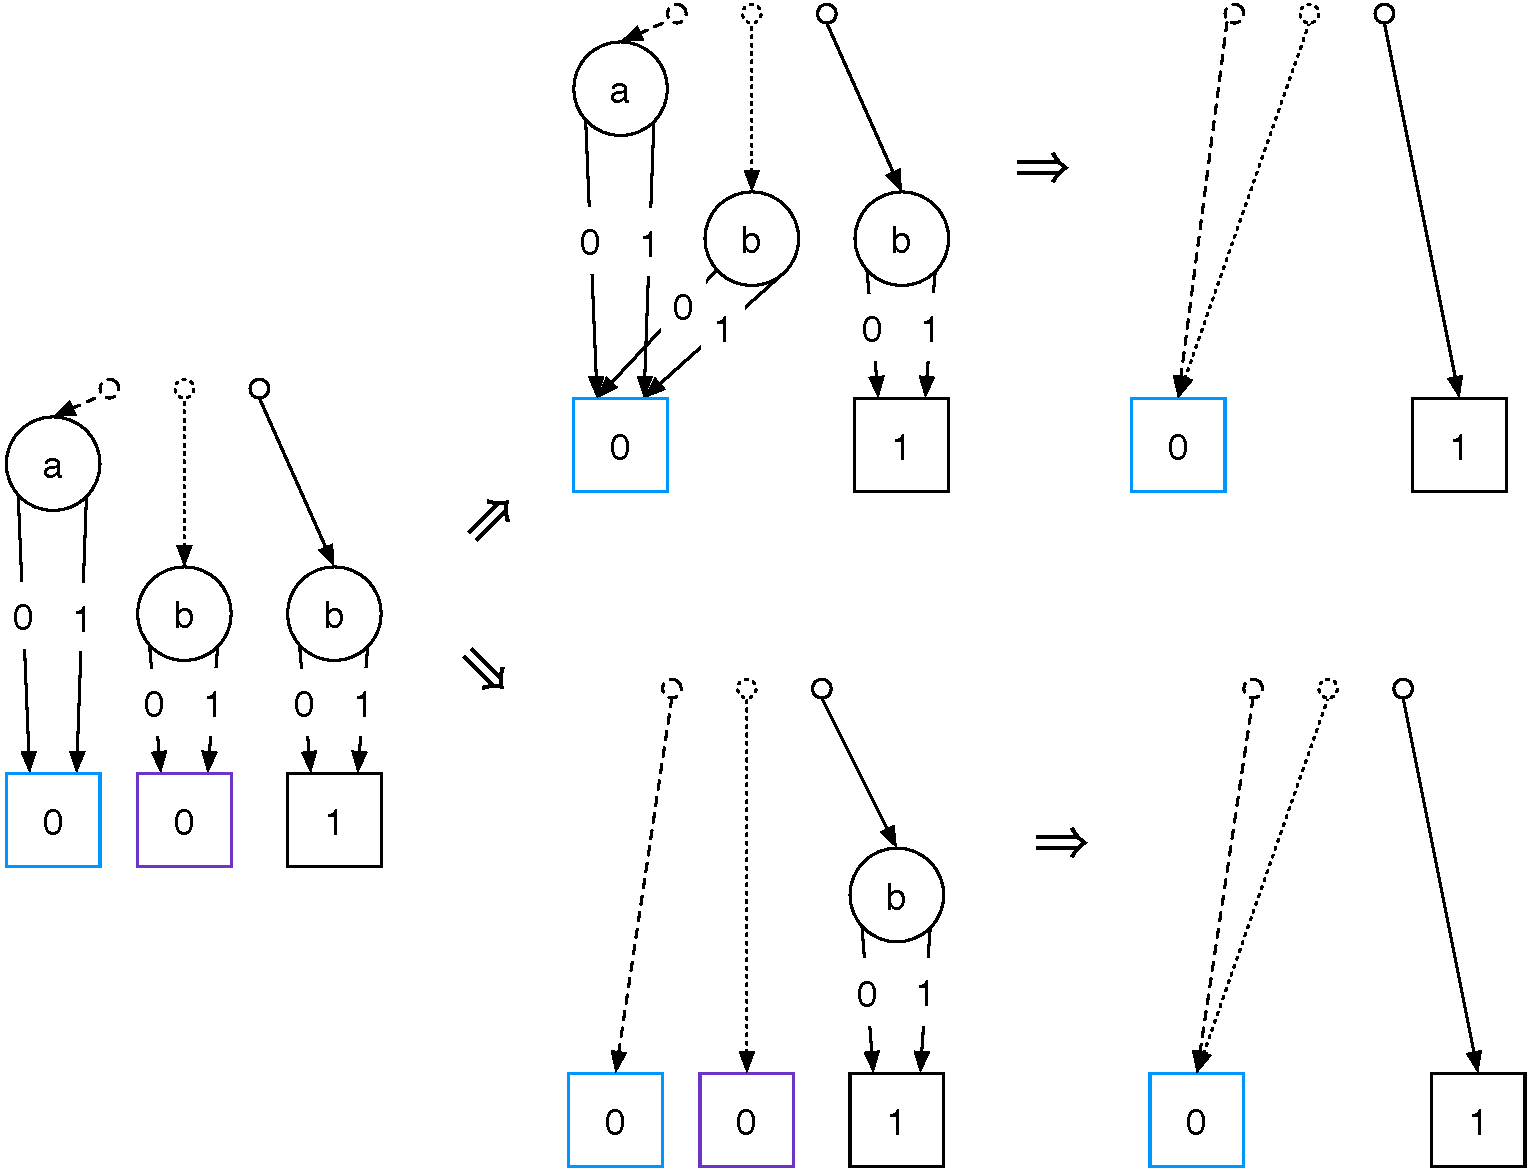
\includegraphics[width=.75\textwidth]{Figures/BDD Removed Terminals And Redundant Tests.pdf}
  \caption{Removal of redundant test and terminal nodes in a BBD}
  \label{fig:Figures_BDD_Removed_Terminals_And_Redundant_Tests}
\end{figure}

Since the removal of redundant test does not change the nodes at the bottom of the tree, all the nodes at the bottom stay. This also means that the reduction works on the same terminal nodes, regardless if we reduce the terminal nodes at the start or after we remove the redundant tests. This in turn means that the order of application does not matter. For an example of this behaviour take a look at Figure~\ref{fig:Figures_BDD_Removed_Terminals_And_Redundant_Tests}.

\paragraph{dn(rt(bdd)) = rt(dn(bdd))}

There is one possibility, where removing redundant tests and redundant nonterminals work on the same part of a BDD. Figure~\ref{fig:Figures_BDD_Removed_Nonterminals_And_Redundant_Tests} shows this possibility. The top part of the graph displays the result if redundant test are removed first. The bottom part shows the result if the redundant nonterminals are removed first. Both times we get the same result. This shows that even if both operations work on the same part of the graph, the application order does not matter.

\begin{figure}[h]
  \centering
    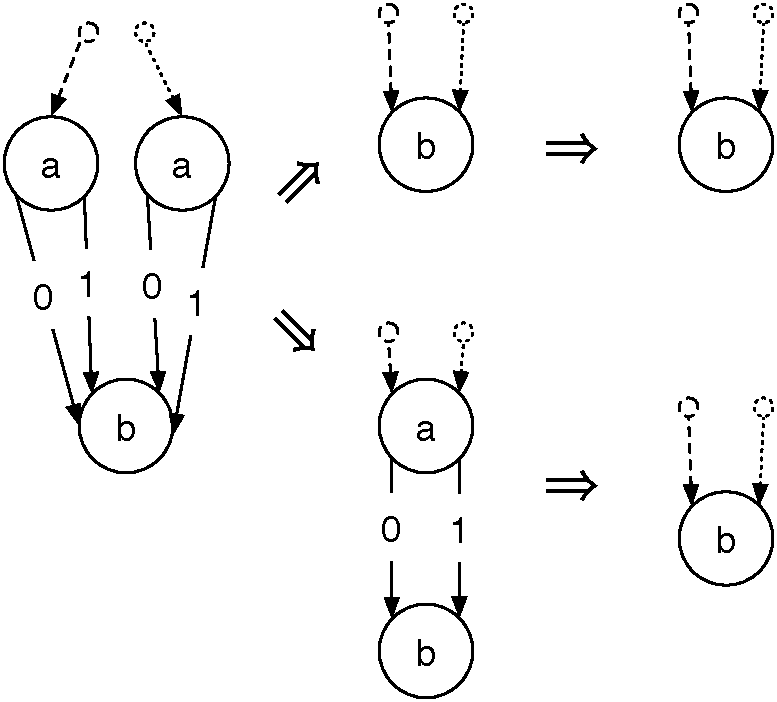
\includegraphics[width=.6\textwidth]{Figures/BDD Removed Nonterminals And Redundant Tests.pdf}
  \caption{Removal of redundant nonterminals and tests}
  \label{fig:Figures_BDD_Removed_Nonterminals_And_Redundant_Tests}
\end{figure}

\newpage
\subsection{Exercise 3}

Describe a size-efficient BDD for the relation “a<b” for n-bit integer numbers.

\subsubsection{Solution}

We assume that:

\begin{itemize}
    \item $a$ has the form $a_na_{n-1}…a_0$, where $a_n$ ist the most significant bit.
    \item $b$ is encoded in the same way as $a$.
    \item Both $a$ and $b$ are positive numbers.
\end{itemize}

Figure~\ref{fig:Figures_OBDD_Smaller} shows the BDD that encodes the boolean operation “a<b”.

\begin{figure}[h]
  \centering
    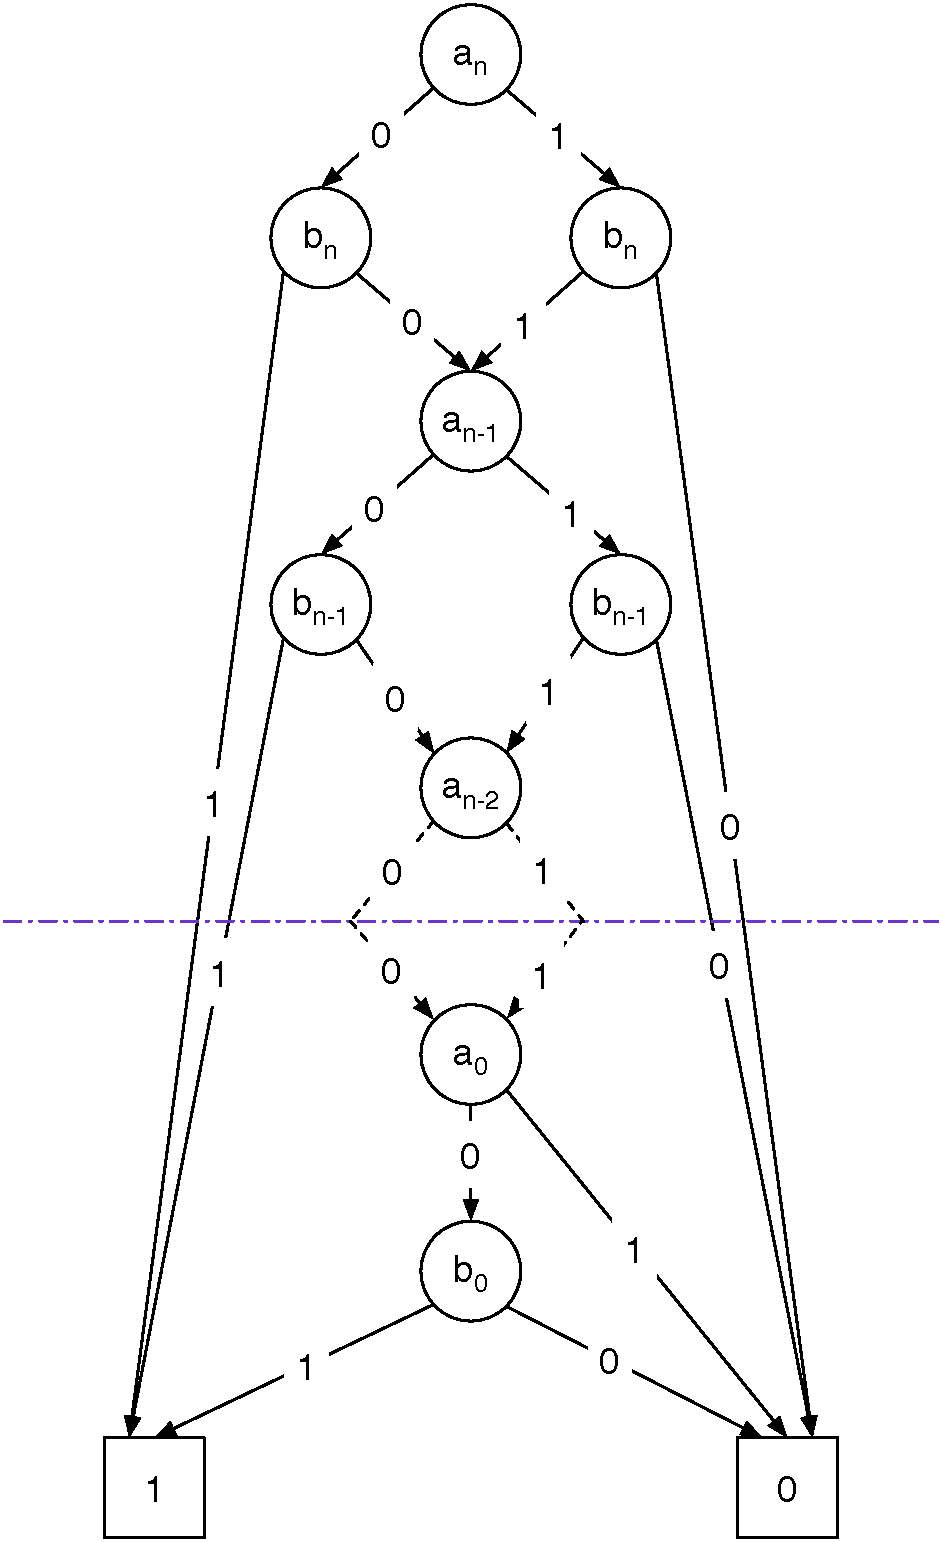
\includegraphics[width=.54\textwidth]{Figures/OBDD Smaller.pdf}
  \caption{An OBBD for the operation “a<b”}
  \label{fig:Figures_OBDD_Smaller}
\end{figure}

\subsection{Exercise 4}

Describe an algorithm which transforms a boolean formula into an equivalent binary decision diagram.

\subsubsection{Solution}

First we need to tokenize and parse the formula. We can use an user friendly parsing library like \href{http://www.dabeaz.com/ply/}{PLY} to do this job. Our basic grammar for formulas would look something like this:

\codeinput{boolean_formula}

The parsing library calls different functions according to the tokens it encounters:

\begin{itemize}
    \item \code{rule\_variable(tokens)}
    \item \code{rule\_constant(tokens)}
    \item \code{rule\_expression(tokens)}
    \item \code{rule\_formula(tokens)}
\end{itemize}

We assume that the functions get a list of the tokens or return values for the matched rule as argument. For example: The (partial) input: $a ∨ 0$ would mean that:

\begin{flushleft}
\begin{itemize}
    \item \code{rule\_variable(tokens)} gets called with \code{tokens = ['a']},

    \item then \code{rule\_constant(tokens)} gets called with \code{tokens = [0]}.

    \item After that, \code{rule\_expression(tokens)} gets called with \code{tokens = [result\_constant, '∨', result\_variable]}.\\[0.5cm]

    \code{result\_constant} and \code{result\_variable} are the values returned by the functions \code{rule\_constant()} and \code{rule\_variable()}.
\end{itemize}
\end{flushleft}

We already defined the parsing process. Now we specify the algorithms used for the parsing functions.

\paragraph{rule\_variable()}

In this rule we create the BDD for the given variable. Figure~\ref{fig:BDD_Variable} shows this simple BDD for the variable $x$.

\begin{figure}[h]
  \centering
    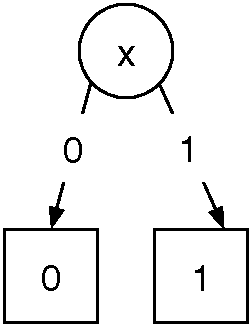
\includegraphics[width=.2\textwidth]{Figures/BDD Variable.pdf}
  \caption{BDD for a single variable $x$}
  \label{fig:BDD_Variable}
\end{figure}

The following listing shows the pseudocode for the function:

\codeinput{rule_variable}

\paragraph{rule\_constant()}

Depending on the given constant we either create the trivial BDD that represents “true” consisting only of the terminal node “1”, or the BDD that only consists of the terminal node “0” representing “false”.

\codeinput{rule_constant}

\paragraph{rule\_expression()}

In this rule \code{tokens} already contains BDDs, since the rules \code{rule\_variable} or \code{rule\_constant} have been executed (for the subformula) before. There are now a few basic possibilities:

\begin{enumerate}
    \item \code{tokens} contains a single BDD returned by the function \code{rule\_constant} or \code{rule\_variable}. In this case we just return the given BDD.
    \item \code{tokens} contains a single BDD and two parenthesis. We just return the BDD.
    \item \code{tokens} contains a not sign ($¬$) followed by an BDD. We invert the tree by swapping the 0- and 1-terminals. After that we return the new BDD.
    \item \code{tokens} contains one BDD, followed by a binary operator and another BDD. In this case we use the function \code{apply} from the lecture slides to create a new BDD.
\end{enumerate}

\codeinput{rule_expression}

\paragraph{rule\_formula()}

This rule already gets the final BDD from the last application of \code{rule\_expression()}. The only thing left to do is to return this BDD.

\codeinput{rule_formula}

\newpage
\section{Temporal Logic}

\subsection{Exercise 5}

Prove the equivalence for $A(f U g)$ on page 16.

\subsubsection{Solution}

We need to prove that $\mathbf{A}(f \mathbf{U} g)$ is equivalent to $¬E(¬g
\mathbf{U} ¬f ∧ ¬g) ∧ ¬\mathbf{EG} ¬g$. We use the following equivalences:

\begin{enumerate}[label=(\arabic*)]
    \item $\mathbf{A} f ⇔ ¬\mathbf{E}¬f$
    \item $¬(f \mathbf{U} g) ⇔ (\mathbf{G}¬g ∨ ¬g \mathbf{U} ¬f ∧ ¬g)$
    The formula above is true since for $f$ until $g$ to not hold:
        \begin{enumerate}

            \item $g$ has to not hold at all (there exists no $k$ such that
            $π^k⊧g$) or

            \item $f$ might hold at first, while $g$ does not hold, but $g$
            does not hold after that ($¬g \mathbf{U} ¬f ∧ ¬g$).

        \end{enumerate}

    \item $\mathbf{E}(f ∨ g) ⇔ \mathbf{E}f ∨ \mathbf{E}g$
    \item $¬ (f ∨ g) ⇔ ¬f ∧ ¬g$
\end{enumerate}

to deduct the following proof:
\begin{align*}
    \mathbf{A}\left(f \mathbf{U} g\right)
    & \stackrel{(1)}{⇔} ¬\mathbf{E} ¬\left(f\mathbf{U} g\right)\\
    & \stackrel{(2)}{⇔} ¬\mathbf{E} \left(\left(\mathbf{G}¬g\right) ∨
      \left(¬g\mathbf{U} ¬f ∧ ¬g\right)\right)\\
    & \stackrel{(3)}{⇔} ¬\left(\mathbf{EG}¬g ∨
      \mathbf{E}\left(¬g\mathbf{U} ¬f ∧ ¬g\right)\right)\\
    & \stackrel{(4)}{⇔} ¬\mathbf{EG}¬g ∧ ¬\mathbf{E}\left(¬g\mathbf{U} ¬f ∧
      ¬g\right)\\
\end{align*}


\subsection{Exercise 6}

Show the following lemma: Let $M$ and $N$ be two Kripke structures such that the transition relation of $M$ is a superset of the transition relation of $N$. If an LTL property $f$ holds on $M$, then $f$ also holds on $N$.

\subsubsection{Solution}

We assume that a certain LTL formula $\mathbf{A}f$ holds on $M$. Since the
transition relation of $M$ is a superset of the transition relations of $N$,
there is always the possibility to construct a Kripke structure equivalent to
$M$ by extending $N$ with additional transitions/states. Since a LTL formula
quantifies over \emph{all paths} in a Kripke structure the set of all formulas
which hold on $N$ gets smaller when we extend $N$. This means that the set of
all LTL formulas which hold on $N$ is a superset of all the LTL formulas which
hold on $M$. From this follows that, if a certain LTL formula $\mathbf{A}f$
holds on $M$, then this formula also has to hold on $N$.


\subsection{Exercise 7}

Show $\mathbf{AFG}~p$ is not logically equivalent to $\mathbf{AFAG}~p$. Which of the two formulas implies the other one?

\subsubsection{Solution}

To show that $\mathbf{AFG}~p$ is not equivalent to $\mathbf{AFAG}~p$ we
construct a Kripke structure which contains a state where $\mathbf{AFG}~p$
holds but $\mathbf{AFAG}~p$ does not.
Figure~\ref{figure:Kripke_Structure_Exercise_6}~\cite{Veith2011ExerciseSolutions} shows this Kripke structure
, where $s₀⊧\mathbf{AFG}~p$ holds, but
$s₀⊧\mathbf{AFAG}~p$ does not.

\begin{figure}[htbp]
    \centering
        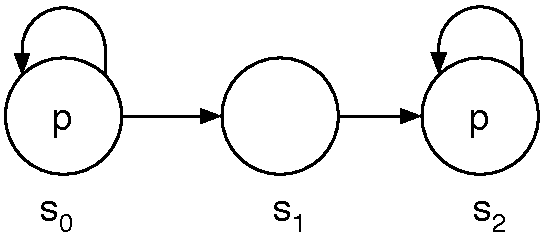
\includegraphics[width=.4\textwidth]
            {Figures/Kripke Structure Exercise 6.pdf}
    \caption{Kripe Structure, where $s₀⊧\mathbf{AFG}~p$ holds, but
             $s₀⊧\mathbf{AFAG}~p$ does not hold}
    \label{figure:Kripke_Structure_Exercise_6}
\end{figure}

\begin{figure}[htbp]
    \centering
        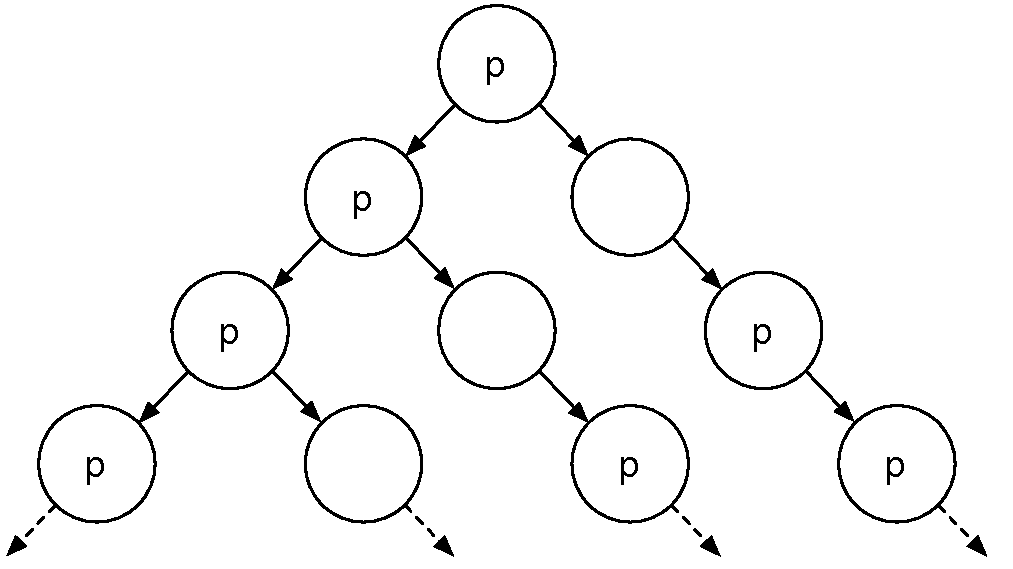
\includegraphics[width=.7\textwidth]
            {Figures/Computation Tree Exercise 6.pdf}
    \caption{Computation Tree for
             Figure~\ref{figure:Kripke_Structure_Exercise_6}}
    \label{figure:Computation_Tree_Exercise_6}
\end{figure}

\begin{description}[style=multiline, leftmargin=3cm]

    \item[$s₀⊧\mathbf{AF}(\mathbf{G}~p)$] This formula specifies that in all
    paths sometimes in the future $p$ will hold globally. This is true for the
    given Kripke structure since we start in $s₀$ in which $p$ holds and either

        \begin{itemize}

            \item continue to stay in this state ($p$ holds globally) or

            \item go to $s₁$ immediately followed by state $s₂$ ($p$ holds
            globally).

        \end{itemize}

    \item[$s₀⊧\mathbf{AF}(\mathbf{AG}~p)$] The formula specifies that
    sometimes in the future for all paths $\mathbf{AG}~p$ (for all paths $p$
    must always be true) has to hold. This is not the case if we follow the
    path on the left in the computation tree for the Kripke Structure (see
    Figure~\ref{figure:Computation_Tree_Exercise_6}) since there is always a
    path on the right where $p$ does not hold for every state.

\end{description}


We already provided an example Kripke structure, where $\mathbf{AFG}~p$ holds but $\mathbf{AFAG}~p$ does not. Since the question “Which of the two formulas implies the other one?” already states that one formula has to imply the other, we conclude that $\mathbf{AFAG}~p$ implies $\mathbf{AFG} p$, since we already disproved $\mathbf{AFG}~p ⇒ \mathbf{AFAG}~p$ with our counterexample.
\subsection{Exercise 8}

Show that all LTL properties have counterexamples which are either finite paths or finite paths which lead to a loop.

\subsubsection{Solution}

One of the standard ways to check an LTL formula is to construct a Büchi
automaton for the negated LTL formula $¬f$ and the given Kripke structure $M$.
These two state machines accept the language $ℒ(¬f)$ respectively $ℒ(M)$. We
now construct a Kripke structure representing the intersection of the two
languages. If the language accepted by this state machine is empty then $M⊧f$
holds. On the other hand, if there exist infinite words accepted by the
automaton, then these words are counterexamples for $M⊧f$.\\

We now need to show that there exists either a finite path or a finite path
with a loop for the language $ℒ(¬f) ∩ ℒ(M)$ if $M⊭f$ is true. We know that if
there exists a counter-example, then there has to be a path in the Büchi
automaton, where at least one acceptance state occurs infinitely often. This
means that this path has to contain a loop. This implies that there has to be
a finite counterexample for $f$, which includes a
loop~\cite{Norrish2010TemporalLogic}.


\subsection{Exercise 9}

Give an LTL specification and a Kripke structure where the smallest counterexample is larger than the number of states in the Kripke structure.

\subsubsection{Solution}

Since there is no restriction on how the Kripke structure should look, we use
the one shown in Figure~\ref{figure:Figures_Kripke_Structure_Exercise_10}.

\begin{minipage}[t]{0.45\textwidth}
    \centering
    \captionof{figure}{A small Kripke structure}
    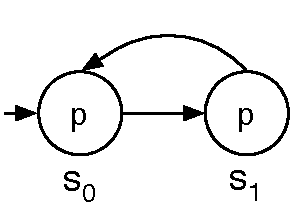
\includegraphics[width=.6\textwidth]
        {Figures/Kripke Structure Exercise 10.pdf}
    \label{figure:Figures_Kripke_Structure_Exercise_10}
\end{minipage}
\begin{minipage}[t]{0.45\textwidth}
    \vskip 1cm
    We use the LTL specification $s₀⊧X(X¬p)$. The smallest counterexample for
    this formula is $s₀, s₁, s₀$.
\end{minipage}


\subsection{Exercise 10}

Show how you can use SMV to solve the Rubik’s cube.

\subsubsection{Solution}

We explain the basic idea behind finding the solution for a small Rubik's cube with only four fields on each side of the cube. The solution for a larger cube can be determined with the same method.\\

We start by drawing the fields of the cube in a 2D plane. Figure~\ref{fig:Figures_Rubik's_Cube_-_2D} shows each field of the cube. We use the numbers on the left and top of the drawing to specify a certain field. This is useful for describing the current state of the fields of the Rubik's cube in SMV. For example we will refer to the leftmost field at the top of the cube shown in Figure~\ref{fig:Figures_Rubik's_Cube_-_2D} as \code{c02} in SMV. Here $0$ specifies the first row and $2$ specifies the third column.

\begin{figure}[h]
  \centering
    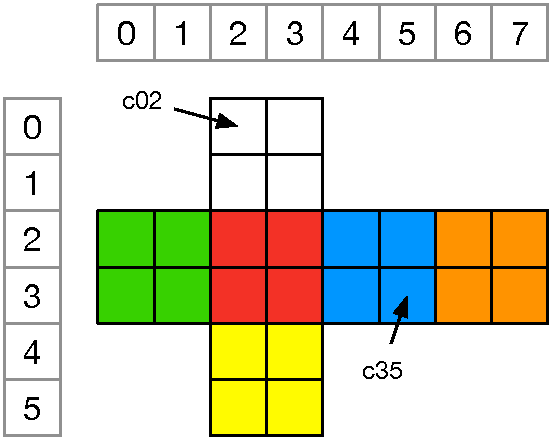
\includegraphics[width=.6\textwidth]{Figures/Rubik's Cube - 2D.pdf}
  \caption{Fields of a small Rubik's Cube}
  \label{fig:Figures_Rubik's_Cube_-_2D}
\end{figure}

We describe the value of a specific field with a certain color in SMV:

\begin{center}
    \code{c02 : \{WHITE, GREEN, RED, BLUE, ORANGE, YELLOW\}; }
\end{center}

For example: The color of field \code{c02} in Figure~\ref{fig:Figures_Rubik's_Cube_-_2D} is \code{WHITE}, the color of field \code{c35} is \code{BLUE}. We now write the module \code{main} and start by defining the variables from \code{c02} upto \code{c53}:

\codeinput{cube_var}

After that, we assign the initial colors (of the unsolved cube) to the fields:

\codeinput{cube_assign}

Now we need to specify the possible transitions of the Rubik's cube from one state to another. For this we assume that we look directly at the cube from a birds eye view. Figure~\ref{fig:Figures_Rubik's_Cube_-_Possibilities} shows that there are eight possibilities for the next move.

\begin{figure}[h]
  \centering
    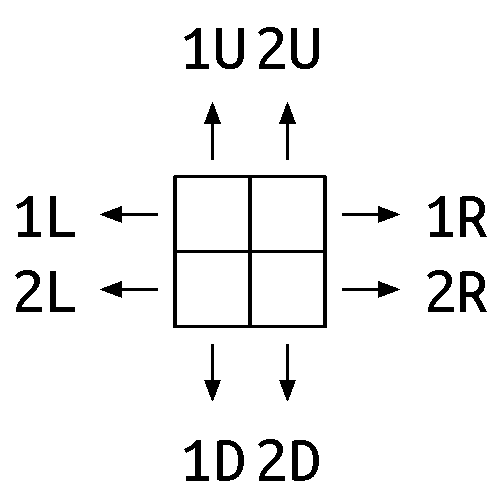
\includegraphics[width=.4\textwidth]{Figures/Rubik's Cube - Possibilities.pdf}
  \caption{Possible moves for a small Rubik's cube}
  \label{fig:Figures_Rubik's_Cube_-_Possibilities}
\end{figure}

To encode each of the possible eight movements we use the SMV keyword \code{TRANS}:

\codeinput{cube_trans}

We now fully specified the initial state of cube and the possible state transitions for the fields of the cube. This leaves us with the question how we can tell SMV to find a solution for our initial cube. For that we define a boolean value \code{solved}, which tells SMV if the cube is solved — the fields of each side have the same color — or not:

\codeinput{cube_define}

We now specify a LTL formula which lets SMV find a possible “path” to a solution. For that we just use the following specification:

\codeinput{cube_spec}

SMV will then find a counterexample for the specified formula $\mathbf{AG} ¬solved $. This counterexample ($¬\mathbf{AG} ¬solved ≡ EF solved$) is a path that describes the state changes of the fields — aka the movements — needed to solve the Rubik's cube with the given default configuration.

\newpage
\section{Questions to Test Your Understanding}

Are the following statements correct/false? Why?

\subsection{Solution}

\begin{enumerate}[label=(\alph*)]
    \item CTL is contained in LTL\\

    This is not the case, since there is not CTL formula that is equal to the LTL formula $\mathbf{AFG}~p$.

    \item LTL is contained in CTL*\\

    This is the case, since CTL* is a superset of both CTL and LTL.

    \item Every CTL formula is equivalent to a formula containing only E, but no A\\

    This is true, since we always can represents a CTL formula of the form $\mathbf{A}~f$ by the equivalent formula $¬\mathbf{E}~¬f$.

    \item Every LTL formula is equivalent to a negation-free formula containing only A, but no E\\

    This is not the case, since the only equivalent representation of the LTL formula $\mathbf{A}~p$ is $¬\mathbf{E}~¬p$, which contains $\mathbf{E}$ and is also not negation-free.

    \item For each Boolean function f over n variables, there exists an order on the variables such that the BDD for f has size linear in n.\\

    No, since there are boolean functions that have exponential size OBDDs for any variable ordering e.g. the middle output of a combinational circuit to multiply two integers.

    \item Every BDD can be translated into an equivalent Boolean formula.\\

    This is true, since a BDD is basically a compact form of a truth table and we can translate a truth table into a boolean formula using a CNF or DNF formula.

    \item On a Kripke structure M, the size of a counterexample is bounded by the number of states in M, multiplied by the size of the specification.\\

    Yes.

    \item Bounded model checking can be used to find the smallest counterexample.\\

    Yes, if there exist a counterexample. To find the smallest counterexample we just start with a bound of 1 and increase it by one till we find a counterexample.

    \item In SMV, each BDD node corresponds to a state in the Kripke structure.\\

    No. BDD nodes usually donate only a part of a specific state — SMV uses BDDs to encode state transitions.

    \item In SMV, BDDs are used as specification language.\\

    No, SMV uses either LTL or CTL as specification language.

\end{enumerate}

% -- Bibliography -------------------------------------------------------------

% Set section format for bibliography
\titleformat{\section}{\sffamily\bfseries}{}{0pt}{}[{\color{aqua}\hrule}]
% Display bibliography
\printbibliography

\end{document}
